\chapter{全局上下文信息与局部信息相结合的异物检测方法}
第三章主要针对地铁屏蔽门与列车门间异物检测应用中首先需要解决的数据集构建及数据标注问题进行了探讨和研究。本章在具有标注数据的前提下,主要研究应用基于深度神经网络的目标检测算法解决地铁屏蔽门与列车门间异物检测的实际问题,分析地铁屏蔽门与列车门间异物图像特征,优化基于聚类算法的锚框生成,同时克服了复杂背景下全局信息利用不足的困难,将其同局部信息有效的结合,提高地铁屏蔽门与列车门间异物检测的精度。

\section{引言}
我国地铁行业高速发展,运营线路、运营线路总长度、客运量等均居世界前列。为了出行方便,越来越多的市民选择地铁作为主要的出行方式,造成客运量越来越大。尤其在早晚高峰时段,车站的人流更是爆满,许多线路在早晚高峰时段列车最大满载率均超过100\%,部分区段高峰小时最达满载率超过120\%,相应的也产生了一些新的交通安全问题。而地铁屏蔽门与列车门间又是连接站台与列车的唯一乘降通道,是地铁系统的风险空间、乘降瓶颈点和管控核心区域。在地铁屏蔽门与列车门间出现异物,即使是细小的手机、雨伞等遗留物,也可能造成灾难性事故,及时发现异物并判断异物类别,可以提升地铁的运输效率和安全保障。在过去,地铁公司大多使用人工瞭望进行检测。然而,人工瞭望这一工作劳动强度大,且准确性易受地铁环境影响,并不能满足地铁系统要求。后来,地铁公司使用红外光幕、激光光幕、激光扫描等光电传感器来进行异物检测。但是,这些光电传感器仍然存在成本高、盲区大、检测效果不理想等缺陷,同样不能很好地满足需求。近年来,随着视频传感器设备及图像处理技术的发展,一些学者开始研究将计算机和图像处理技术应用于地铁屏蔽门与列车门间的异物检测。当前存在两种形式的视频检测系统:侧装式及顶装式。在检测盲区方面,侧装式系统仍然会存在一定的盲区。而在检测算法方面,侧装式及一部分顶装式检测系统中仍采用背景建模及模板匹配等传统图像处理算法,需人工设计特征且鲁棒性不强,极易受到外界环境影响,且不能自动判断出异物类别,需工作人员进行二次识别,效率低下。因此,使用顶装式检测系统,并改进地铁屏蔽门与列车门间异物检测系统的图像识别算法,提高异物检测精度,实现异物的自动检测具有重要的意义。

\section{问题分析}
地铁屏蔽门与列车门间是连接站台与列车的唯一乘降通道,情况复杂,人员众多,在两门开启关闭过程中,容易出现异物遗留的情况,如手机、雨伞、钱包,乘客等,若不及时发现及处理异物,将会影响地铁列车的正常工作,导致乘客人身安全及地铁运行安全受到威胁。据统计\cite{刘伟铭2019地铁风险空间分析及异物检测系统技术要求},某城市地铁站在2017年发生造成延误的异物事件共101起,各事件的比例按从大到小排列,如图\ref{异物事件比例}所示:(1)大部分异物事件为雨伞、水瓶、钱包等小异物体遗落站台边缘,占比 35.87\%;(2)由于客流拥挤,列车门启动防夹功能事件,占比 16.30\%;(3)列车门与屏蔽门夹乘客手指、手臂、头发等事件,占比16.30\%;(4)乘客背包包带被夹事件,占比14.13\%;(5)乘客衣服被夹事件,占比9.78\%;(6)最后,其他微小异物(如瓶盖、金属徽章、佛珠等)遗留事件,占比 7.61\%。
\begin{figure}[htbp]
	\centering
	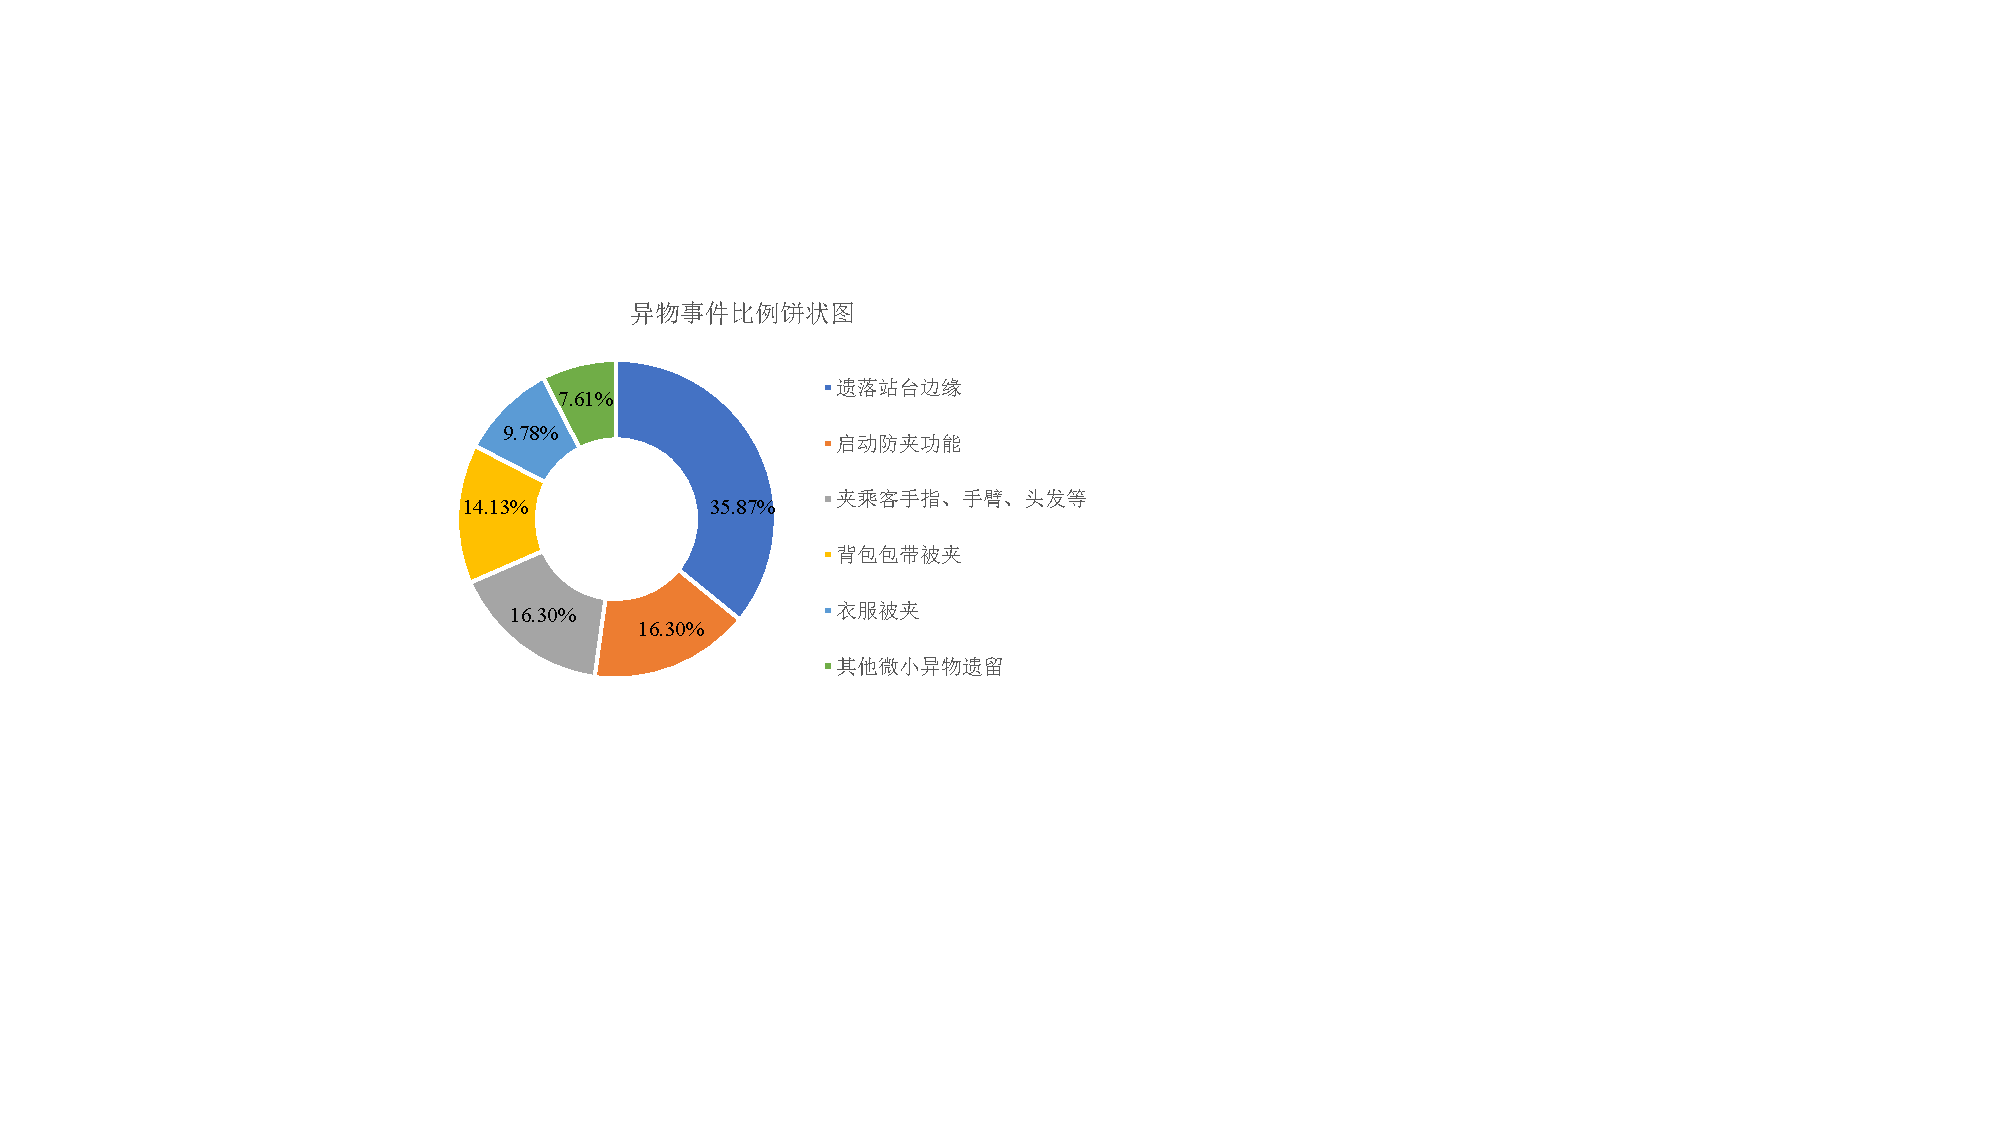
\includegraphics[scale=1]{Fig/异物比例.pdf}
	\caption{\label{异物事件比例}地铁屏蔽门与列车门间异物事件比例}
\end{figure}

本章以地铁屏蔽门与列车门间异物检测为主要研究任务,该任务存在两个主要的特点:
\begin{enumerate}[topsep = 0 pt, itemsep= 0 pt, parsep=0pt, partopsep=0pt, leftmargin=44pt, itemindent=0pt, labelsep=6pt, label=(\arabic*)]
	\item 现有基于锚框的深度学习目标检测算法在锚框生成这一步骤中,通常存在两种生成方法,手工方法和聚类方法:手工方法即为手工挑选锚框的尺寸,而聚类方法则通常是使用K-means 聚类算法自动找到良好的锚框。然而,这两种方法均存在一定的缺陷:手工方法需要人工挑选,工作强度较大,网络虽然可以通过学习适当地调整锚框形状,但是如果从一开始就为网络选择更好的锚框,就可以让网络更容易学习并获得更好的检测结果。而使用K-means聚类算法来生成锚框则受限于K-means 聚类算法本身的局限性,聚类结果很容易受到初始值的选取影响。因此,如何更好地自动生成锚框是第一个挑战。
	
	\item 以VGGNet\cite{vggnet}、InceptionNet系列\cite{Inceptionv1,Inceptionv2,Inceptionv4}和 ResNet系列\cite{resnetv1,resnetv2,resnetv3}为代表的卷积神经网络 (ConvNets)在多种视觉任务中取得了巨大的进展,它们的共同特点是顺序堆叠多个基本模块,并采用金字塔结构,但是却忽略了显式建模全局上下文信息的重要性。自从 2020 年以来,视觉 Transformer\cite{ViT,detr,Deformable-detr}进一步促进了视觉识别模型的发展,在ImageNet图像分类和下游任务上表现出比最先进的ConvNets更好的结果。这是因为与只进行局部建模的卷积操作相比,Transformer中的自注意力机制能够对全局的成对依赖进行建模,提供了一种更有效的空间信息编码方法。然而,在处理高分辨率图像时,自注意力机制导致的计算成本是相当大的。同时,许多研究\cite{Inside-OutsideNet,Combining-Multiple-Sensors-for-Event-Detection-of-Older-People,Attentive-Contexts-for-Object-Detection}已经证实,全局上下文信息可以为目标检测带来性能提升。在地铁这一复杂巨系统中,全局上下文信息对于异物检测同样也是至关重要的。因此,如何将Transformer擅于捕捉长距离依赖关系和ConvNets擅于提取局部特征这两个优点强强联手,在基于CNN的深度学习目标检测算法中有效的利用全局上下文信息,且不会大量增加模型的计算成本是第二个挑战。
\end{enumerate}

\section{异物检测模型GL-YOLO}
目标检测,是通过分析目标的几何特征,从图像或视频中定位感兴趣的目标,准确地判断每个目标的具体类别,并给出每个目标的边界框。近年来,深度卷积神经网络依靠其不仅能够提取高层特征,提高特征的表达能力,还能够将特征提取、特征选择和特征分类融合在同一个模型中,通过端到端的训练,从整体上进行功能优化,增强特征的可分性等优点推动目标检测领域取得了重大进展。

基于深度卷积神经网络的目标检测算法大致可分为两类:双阶段目标检测算法和单阶段目标检测算法。双阶段目标检测算法先根据图像提取候选框,然后基于候选区域做二次修正得到检测点结果,检测精度较高,但检测速度较慢。这类算法的开山之作是R-CNN\cite{rcnn},随后Fast-RCNN\cite{fastrcnn}、Faster-RCNN\cite{fasterrcnn}依次对其进行了改进。由于优秀的性能,Faster-RCNN至今仍然是目标检测领域很有竞争力的算法。随后,FPN\cite{FPN}、Mask-RCNN\cite{maskrcnn}等算法又针对Faster-RCNN的不足提出了改进,这进一步丰富了Faster-RCNN的组件,提升了它的性能。相较于双阶段目标检测算法,单阶段目标检测算法直接对图像进行计算生成检测结果,检测低速度快,但检测精度较低。这类算法的开山之作是YOLO\cite{yolov1,yolov2,yolov3},随后SSD\cite{SSD}、Retinanet\cite{retinanet}依次对其进行了改进,后续有团队将一些有助于提升性能的技巧融入到YOLO系列算法中,在YOLOv3的基础上又提出了4个改进版本:YOLOv4~YOLOv7\cite{YOLOv4,glenn_jocher_2021_4679653,YOLOv6,yolov7}。由于后续各类技巧的融合,使得YOLO系列的检测准确率有了很大的进步,同时由于较快的运行速度,YOLO系列算法成为了工业界的主流。

对于目标检测任务而言,理论上讲,各个目标之间的关系是有助于提升目标检测效果的。然而基于卷积神经网络的目标检测算法,无论是单阶段还是双阶段目标检测,都没有很好地利用到注意力机制。针对这种情况,Relation Net\cite{Relationnet}和DETR\cite{detr}利用Transformer将注意力机制引入到目标检测领域。Relation Net利用Transformer对不同目标之间的关系建模,在特征之中融入了关系信息,实现了特征增强。DETR则是基于Transformer提出了全新的目标检测架构,开启了目标检测的新时代。

本章提出的地铁屏蔽门与列车门间异物检测模型采用基于YOLOv5的目标检测方法,实现异物的自动检测,同时克服了传统YOLOv5模型对于全局上下文信息利用不足的缺陷,提高异物检测的精度。基于YOLOv5的地铁屏蔽门与列车门间异物检测模型结构GL-YOLO如图4-2所示,该模型以YOLOv5算法为基础,为了解决原始YOLOv5对于全局上下文信息利用不足而导致精度不高的问题,在基于YOLOv5算法的基础上引入Transformer和注意力机制,将原始YOLOv5中的卷积模块同Transformer和注意力机制相结合,使得模型有效的利用了局部信息和全局上下文信息;同时,使用K-Means++聚类算法代替K-Means聚类算法来生成锚框,缓解K-Means聚类算法收敛情况严重依赖于簇中心的初始化状况,从而一定程度上提高了检测精度和效果。
\begin{figure}[htbp]
	\centering
	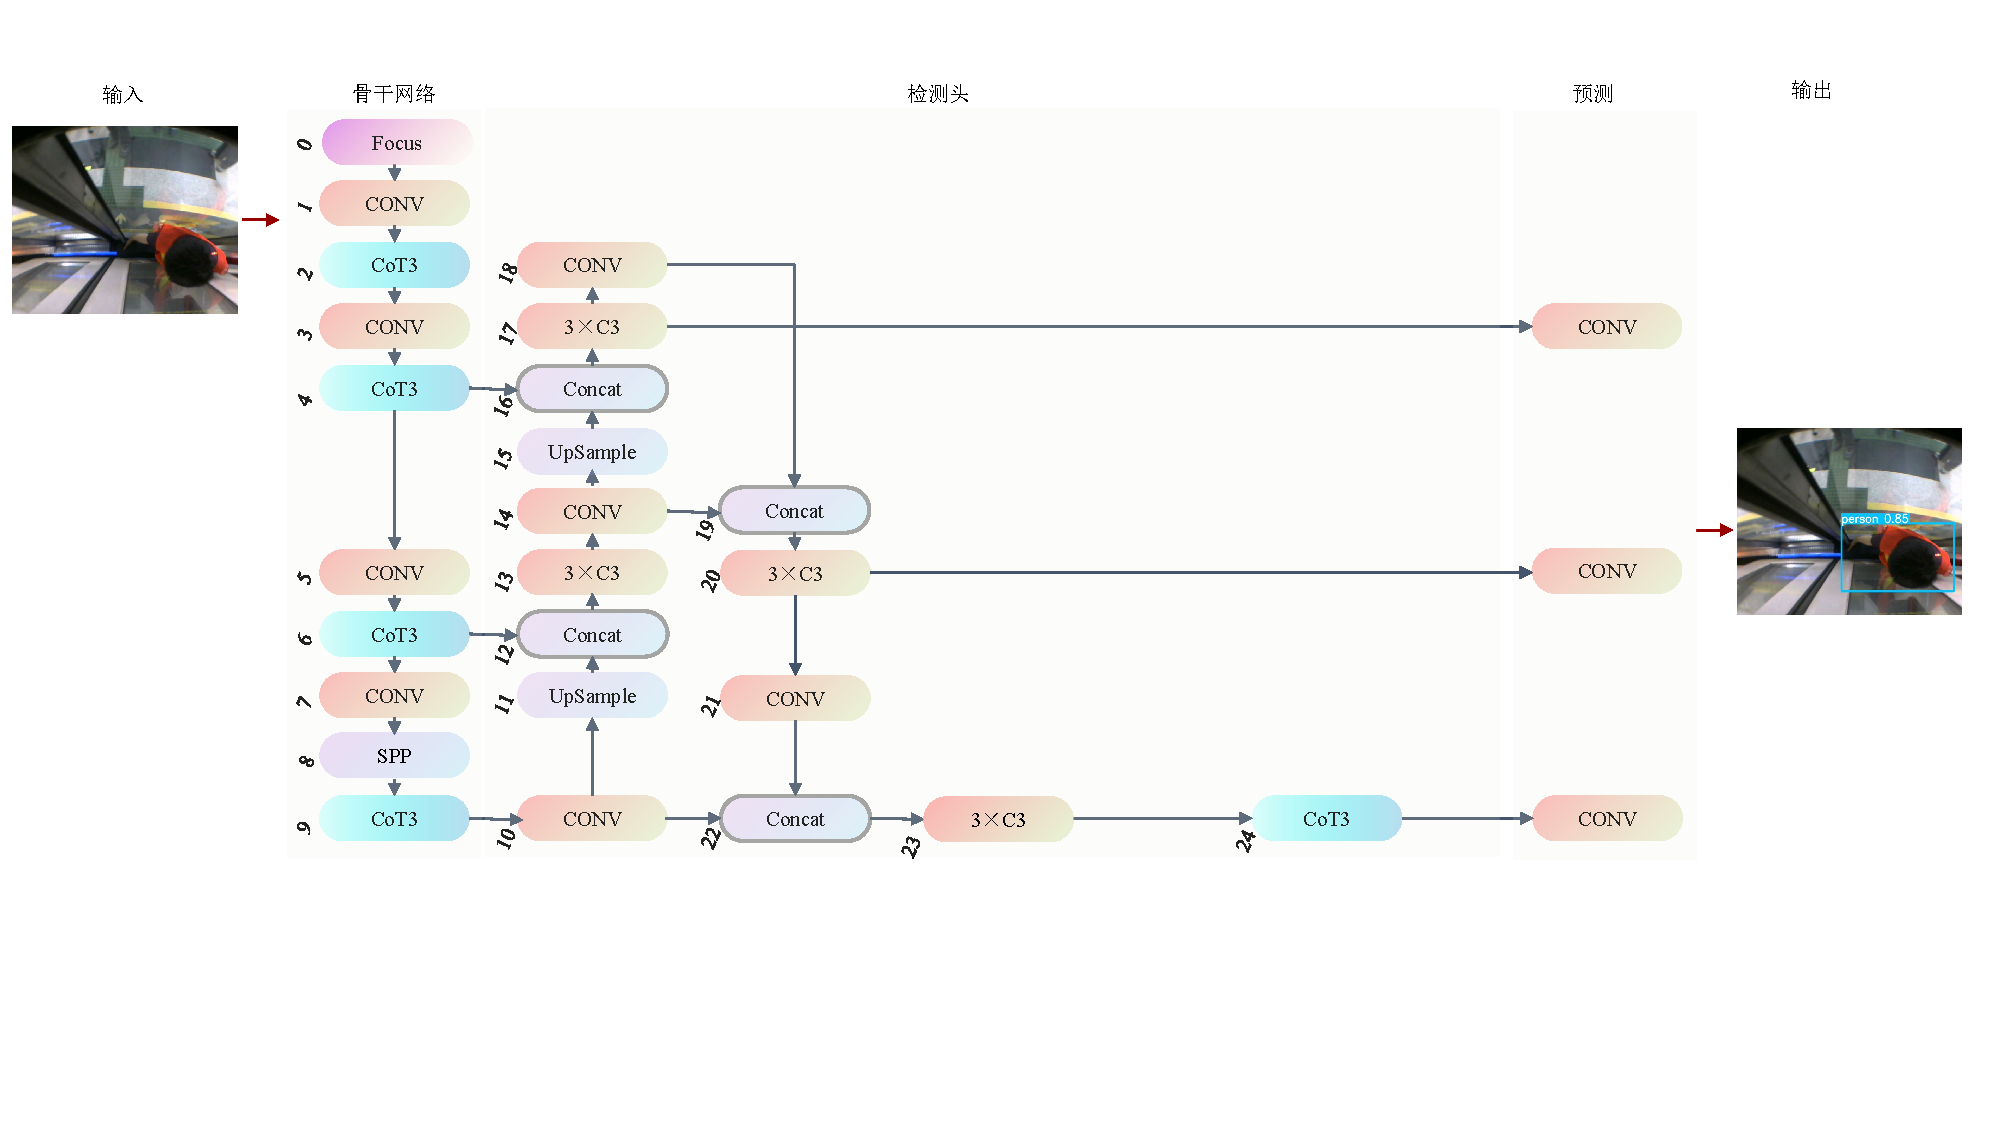
\includegraphics[scale=0.5]{Fig/GL-YOLO.pdf}
	\caption{\label{GL-YOLO}地铁屏蔽门与列车门间异物检测模型GL-YOLO结构}
\end{figure}

\subsection{基于K-Means++的锚框生成}
近年来,基于深度卷积神经网络的目标检测算法取得了长足的进步。虽然目前出现了一些无锚框算法, 但是锚框机制仍然被广泛用于最先进的目标检测框架中,并在常用公开数据集(例如PASCAL VOC和MSCOCO)上取得突出效果。

锚框实际上是一组预定义的边框,在训练时,使用真实的边框位置相对于预定义边框的偏移来构建训练样本,简单理解为最开始在图像中有可能的位置将目标框出来,然后在这些预定义边框的基础上进行调整。在目标检测框架中生成锚框的最直接的方法是通过枚举,现有的锚框生成方法可以分为两类:手工方法和聚类方法。手工方法主要是基于先前的经验来确定锚框的大小和长宽比,比如SSD和Faster-RCNN算法中对锚框的设置。手工方法设置锚框的不足是锚框的尺寸往往会和数据集中目标的大小存在差异,从而影响检测效果。聚类方法是基于特定的数据集用聚类算法去计算锚框最合适的大小和长宽比。聚类指的是把集合,分组成多个类,每个类中的对象都是彼此相似的。K-Means是聚类中最常用的方法之一,它是基于点与点距离的相似度来计算最佳类别归属。YOLOv2是最先使用K-Means算法来对数据集进行聚类,生成锚框的算法。到后续的YOLOv3也是在MS COCO数据集上使用K-Means算法进行聚类,生成锚框,最终选择(10$\times$13), (16$\times$30), (33$\times$23), (30$\times$61), (62$\times$45), (59$\times$119), (116$\times$90), (156$\times$198), (373$\times$326),这9个聚类结果作为先验。YOLOv5也是默认采用K-Means算法聚类COCO数据集来生成锚框,并在训练过程中采用遗传算法调整锚框。

K-Means算法的输入为数据集的标注文件,本文中所使用数据集的标注文件均为.xml格式,其中包含目标的类别信息,图片的宽、高、深度即(width、height、depth)信息,以及目标的先验bounding box的坐标值,即$(x_{min},y_{min})$和$(x_{max},y_{max})$。值得注意的是,标准的K-Means是用欧式距离来衡量相似度的,然而这个衡量标准在锚框生成中是不合适的,因为使用欧氏距离来衡量相似度,在bounding box尺寸比较大的时候,误差也更大。而我们在锚框生成过程中希望的是误差和尺寸没有太大关系。因此,在锚框生成过程中,需要弃用欧氏距离,而通过求取bounding box之间的交并比(Intersection over Union, IoU)即面积比来衡量相似度。具体求解公式如下所示:
\begin{equation}
	d(box,centroid)=1-\mathrm{IoU}(box, centroid)
	\label{Iou}
\end{equation} 

因此,使用K-Means聚类算法来生成锚框的伪代码如下表\ref{K-Means}所示。K-Means算法的优点是速度快,实现简单。但是K-Means在聚类时,从其算法的原理可知,K-Means正式聚类之前首先需要完成的就是初始化个簇中心。同时,也正是因为这个原因,使得K-Means聚类算法存在着一个巨大的缺陷:收敛情况严重依赖于簇中心的初始化状况,最终结果跟初始点选择相关,容易陷入局部最优。针对此种情况,本文弃用K-Means算法,转而K-Means++聚类算法来生成锚框。使用K-Means聚类算法来生成锚框的伪代码如表\ref{K-Means++}所示。
\begin{table}[htbp]
	\centering
	\caption{K-Means聚类算法生成锚框伪代码}
	\scalebox{0.7}{
	\begin{tabular}{cl}
		\toprule[2pt]
		1:  & 随机设定初始聚类中心; \\
		2: & 利用公式\ref{Iou}计算距离,将距离某个聚类中心距离近的样本点归类到该聚类中心,将样本全部归类完毕后得到多个簇 \\
		3:     & 计算每个簇的均值作为新的聚类中心; \\
		4:    & 重复第2步和第3步,直至聚类中心不再发生变化。 \\
		\bottomrule[2pt]
	\end{tabular}
}%
	\label{K-Means}%
\end{table}%
\begin{table}[htbp]
	\centering
	\caption{K-Means++聚类算法生成锚框伪代码}
	\scalebox{0.7}{
		\begin{tabular}{cl}
			\toprule[2pt]
			1:  & 从输入的数据集中随机选取一个点作为第一个中心点; \\
			2: & 对每一个点分别计算到已选取的中心点的距离 \\
			3:     & 按照轮盘法选择一个新的点作为新的中心点,选取的原则是:距离较大的点,有较大的概率被选取; \\
			4:    & 重复步骤2,3直到K个中心点被选出; \\
			5:    & 利用这K个中心点作为初始点执行K-means算法。 \\
			\bottomrule[2pt]
		\end{tabular}
	}%
	\label{K-Means++}%
\end{table}%

对比表\ref{K-Means}和表\ref{K-Means++},可以看出,K-Means++算法实际就是修改了K-Means算法的第一步操作,之所以进行这样的优化,是为了让随机选取的中心点不再只是趋于局部最优解,而是让其尽可能的趋于全局最优解。因此,采用K-Means++可以有效缓解K-Means算法的问题,生成质量更高的锚框,从而一定程度上能够提高检测精度和效果。

\subsection{全局上下文信息与局部信息的结合}
如何较好的引入全局信息,而不造成太多计算量增加。以 VGGNet、Inception 系列和 ResNet 系列为代表的 2010-2020 年代的卷积神经网络 (ConvNets) 在多种视觉任务中取得了巨大的进展,它们的共同特点是顺序堆叠多个基本模块 (Basic Building Block),并采用金字塔结构 (pyramid network architecture),但是却忽略了显式建模全局上下文信息的重要性。SENet 模块系列模型突破了传统的 CNN 设计思路,将注意力机制引入到 CNN 中以捕获远程依赖,获得了更好的性能。

自从 2020 年以来,视觉 Transformer (ViTs) 进一步促进了视觉识别模型的发展,在 ImageNet 图像分类和下游任务上表现出比最先进的 ConvNets 更好的结果。这是因为与只进行局部建模的卷积操作相比,Transformer 中的自注意力机制能够对全局的成对依赖进行建模,提供了一种更有效的空间信息编码方法。然而,在处理高分辨率图像时,自注意力机制导致的计算成本是相当大的。许多研究表明,目标周围的背景信息对于提升目标检测的精度有着积极意义。而在地铁这一复杂巨系统中,上下文信息对于异物检测同样至关重要。然而,目前许多目标检测算法对于全局上下文信息的利用还不够充分:基于CNN的算法受限于感受野,缺乏全局建模的能力;而最近的基于Transformer的算法擅长于捕获长局依赖关系但是在局部特征采集上却力有未逮,因此限制了检测的精度。本章为了提升对异物的检测准确率,重点研究将全局上下文信息与局部信息相结合利用的目标检测方法。当前一些广泛使用的基于卷积神经网络的目标检测算法,如SSD[12]、YOLOv3-5[13-15]等在定位目标时仅使用候选目标区域内部的特征信息,而捕获全局上下文信息的能力不足。然而,一些研究[16-18]已经证实,全局上下文信息也可以为目标检测带来性能提升。例如,如果想要检测一张图片中的特定汽车,通常与目标同时出现的物体(比如人、道路或另1辆车)可能会为检测目标提供有用的线索。因此,全局上下文信息可以与局部信息相结合,为目标检测提供有用的指导。具体到地铁屏蔽门与列车门间异物检测这一任务,以图1来对使用全局上下文信息同局部信息相结合来进行异物检测这一过程进行说明:图1(a)中3个语义相关性更强的位置(1个真实的塑料袋及其2个倒影)拥有更高的置信度。同时,可能会影响模型检测性能的背景噪声被成功抑制。然后,将图1(a)中的全局上下文信息同图1(b)中的局部信息相结合,引导模型成功检测到异物(图1(c))。YOLOv5s在检测过程中只利用候选目标区域内部的特征进行检测。然而,对于整张图片来说,背景有时候也能够提供有用的信息。例如,如果想要检测1张图片中的特定汽车,通常与目标同时出现的物体(例如人、道路或另1辆车)可能会为检测目标提供有用的线索。当然,并不是所有的背景信息都有利于提高目标检测性能,一些无意义的背景噪声可能会损害检测性能。因此,如何有效的利用全局上下文信息是一个值得研究的问题。
大部分能够对全局上下文进行建模的注意力机制用于深度神经网络通常可以带来很好的性能提升,但将这些注意力机制应用于规模较小的网络中时,最终表现却不如将注意力机制应用于规模较大的深度神经网络。这主要是对于规模较小的网络来说,相比于引入注意力机制带来的效果提升,同时增加的大量运算是更无法接受的。以非局部[24]模块(如图4a)为例:非局部模块使用自注意力机制来对远程依赖进行建模。对于每个查询点,非局部模块首先计算查询点与所有点之间的成对关系以得到注意力图,然后通过加权和的方式聚合所有点的特征,从而得到与此查询点相关的全局特征,最终再分别将全局特征加到每个查询点的特征中,完成远程依赖的建模过程。非局部模块的这种操作,虽然有利于提升模型的检测效果,然而却导致了运算量过大的问题。同时,模型可以将这些全局上下文信息同局部特征信息相结合去检测异物,最终在提升模型检测效果的同时也不会大量增加模型的运算量。


\subsection{损失函数}

\section{实验与结果分析}
\subsection{实验数据集}
为了评估本章所提出算法GL-YOLO的性能,将在公开数据集PASCAL VOC及第三章所构建的FODD这两个数据集上同其他先进检测模型进行对比实验。
\subsubsection*{(1) PASCAL VOC}
PASCAL VOC\cite{pascalvoc07, pascalvoc12}是一个常用的分类、识别和检测视觉目标的基准数据集。它的特点是包含多样化的场景以及多种物体类别。PASCAL VOC提供了一整套从数据标注到算法评估的标准流程,它采用了一种名为xml的标注方法,数据集中的每一张图片对应一个xml格式的文件,其中包含了该图片的名称、图片尺寸、物体类型、位置、大小、是否完整和预测难度等信息。PASCAL VOC(2005-2012)竞赛的目标主要是进行图像目标检测,数据集中包含了生活中常见的20种物体,包括飞机、自行车、鸟、船、瓶子、公共汽车、小汽车、猫、椅子、奶牛、餐桌、狗、马、摩托车、人、盆栽、羊、沙发、火车和显示器。

PASCAL VOC有两个版本的数据集:VOC2007和VOC2012。VOC2007包含9963张标注过的图片,由train/val/test三部分组成,共标注出24,640个物体。而VOC2012是VOC2007数据集的升级版,一共有11530张图片。VOC2012的trainval/test包含08-11年的所有对应图片,并与VOC2007互斥,trainval中有11540张图片,共27450个物体。VOC2007和VOC2012数据集及二者的并集数据量对比如下表所示。
\begin{table}[htbp]
	\centering
	\small
	\caption{PASCAL VOC数据集详细信息}
	\setlength{\tabcolsep}{1.3mm}
	\begin{tabular}{ccccccccccc}
		\toprule[2pt]
		\multirow{2}[4]{*}{} & \multicolumn{2}{c}{训练集} & \multicolumn{2}{c}{验证集} & \multicolumn{2}{c}{训练与验证集} & \multicolumn{2}{c}{测试集} & \multicolumn{2}{c}{全部} \\
		\cmidrule{2-11}          & 图片数   & 目标数   & 图片数   & 目标数   & 图片数   & 目标数   & 图片数   & 目标数   & 图片数   & 目标数 \\
		\midrule
		VOC07 & 2501  & 6301  & 2510  & 6307  & 5011  & 12608 & 4952  & 12032 & 9963  & 24640 \\
		VOC12 & 5717  & 13609 & 5823  & 13841 & 11540 & 27450 & {\color{red} 11540} & {\color{red} 27450} & {\color{red} 23080} & {\color{red} 54900} \\
		总计    & 8218  & 19910 & 8333  & 20148 & 16551 & 40058 & {\color{red} 16492} & {\color{red} 39482} & {\color{red} 33043} & {\color{red} 79540} \\
		\bottomrule[2pt]
	\end{tabular}%
	\label{pascal voc}%
\end{table}%

表中,黑色字体所示数字是官方给定的,由于VOC2012数据集中测试集部分没有公布,因此红色字体所示数字为估计数据,按照PASCAL VOC通常的划分方法,即训练与验证集与测试集各占总数据量的一半。在后续的实验中,本章使用VOC2007的训练集+验证集和VOC2012的训练集+验证集训练,然后使用VOC2007的测试集测试,即在大多数论文中经常看到的07+12方法。
\subsubsection*{(2) FODD}

\subsection{评价指标}
在目标检测领域,均值平均精度(mean Average Precision, mAP)和每秒传输帧数(Frame Per Second, FPS)这两个评价指标是衡量目标检测算法准确性及检测速度的权威指标,被广泛应用于评价目标检测算法的性能。此外,由于本文所研究算法将面向实际应用,需要考虑到具体的硬件设备算力。因此,本文在此还将添加模型参数量(Parameters)、运算量(GFLOPs)作为额外的评价指标。下面给出这四个评价指标的具体计算方式:
\subsubsection*{(1) mAP}
\subsubsection*{(2) FPS}
\subsubsection*{(3) Parameters}
\subsubsection*{(4) GFLOPs}
\subsection{实验环境及超参数设置}
\subsection{FODD上的实验结果}
\subsection{PASCAL VOC上的实验结果}
\subsection{消融实验}

\section{本章小结}
